\documentclass[onecolumn]{aastex62}


\newcommand{\vdag}{(v)^\dagger}
\newcommand\aastex{AAS\TeX}
\newcommand\latex{La\TeX}
\usepackage{listings}
\usepackage{amsmath}
\usepackage{physics}
\usepackage{hyperref}
\usepackage{natbib}
\usepackage[T1]{fontenc}
\usepackage[english]{babel}
\usepackage[utf8]{inputenc}

\begin{document}

\title{\Large Milestone II:\\Studying the recombination history of the universe.}


\author{Håkon Tansem}

\section{Introduction} \label{sec:intro}
This is the second out of four milestones in a project where the final goal is to compute the CMB power spectrum. Previously, in milestone I \cite{TansemI:2020}, we calculated the background evolution of the universe studying how the energy content and the particle horizon has evolved throughout cosmic history. Another important consideration to take into account when observing the CMB is to study the medium the photons have travelled from their release at the last scattering surface untill they reach us at present time. In this second milestone we will study how the optical depth of the universe changes as we look further back in time. To do this we will have to study the recombination history of the universe; i.e how the fraction of ionized matter versus neutral matter has changed during the history of the universe. 
\section{Method} \label{sec:method}
The general expression for optical depth $\tau$ is given by
\begin{equation}
    d\tau\equiv\alpha(s)ds,
\end{equation}
where $\alpha(s)$ is the attenuation coefficient and $s$ is the thickness of the medium. When considering the intergalactic medium the CMB photons have traversed untill we observe them, the main contributor to the attenuation coefficient is thomson scattering off free electrons. The expression for optical depth $\tau$ can then be written as
\begin{equation}
    d\tau=n_e\sigma_T ad\eta,
\end{equation}
where $n_e$ is the free electron density, $a$ is the scale factor and $\sigma_T = \frac{8\pi}{3}\frac{\alpha^2\hbar^2}{m_e^2c^2}$ is the Thomson scattering cross-section, where $\alpha$ is the fine structure constant, and $m_e$ is the electron mass. We have now also changed coordinates to the conformal time $\eta$ representing the thickness of the medium. By performing a change of coordinates to $x=log(a)$ we can get a differential equation for $\tau$ given by
\begin{equation}\label{eq:optical_depth_of_x}
    \frac{d\tau}{dx} = -\frac{n_e \sigma_T }{H(x)},
\end{equation}
where $H(x)$ is the Hubble parameter in our new coordinate system. The evolution of the Hubble parameter used in the calculation is described in milestone I. To solve the ODE for $\tau$ we need to evaluate the electron density $n_e$ as a function of $x=log(a)$. When studying the recombination history of the universe, our model will include some simplifications. In this project we will mostly study the phenomenon of recombination and ignore the reionization the universe went through later. We assume the universe mostly consists of hydrogen by setting the helium fraction $Y_p=0$. We also assume that all baryonic matter is represented by the hydrogen nucleus. This makes us able to approximate the proton density $n_H$ as
\begin{equation}\label{eq:baryondensity}
    n_H = n_b \approx \frac{\rho_b}{m_H} = \frac{\Omega_{b,0} \rho_{c,0}}{m_H a^3},
\end{equation}
where $n_b$ is the baryon density, $\rho_{c,0}$ is the critical density of the universe today, $\Omega_{b,0}$ is the density parameter for baryons today and $m_H$ is the hyodrogen mass. A relationship between the quantities $n_e$ and $n_H$ can be expressed through the free electron fraction given by

\begin{equation}\label{eq:Xe}
    X_e\equiv\frac{n_e}{n_H}.
\end{equation}
 
This allows us to solve for $n_e$ to compute the optical depth given in equation \ref{eq:optical_depth_of_x}. The free electron fraction can be solved using two equations dependent on quantities that evolve with $x=log(a)$. The first one is the Saha equation given by
\begin{equation}\label{eq:saha_eq}
    \frac{X_e^2}{1-X_e} = \frac{1}{n_b} \left(\frac{m_eT_b}{2\pi}\right)^{3/2} e^{-\epsilon_0/T_b},
\end{equation}
where $\epsilon_0=13.6$eV is the ionization energy of the hydrogen atom, $m_e$ is the electron mass and $T_b$ is the baryon temperature. The baryon temperature can be approximated by the photon temperature giving $T_b =
T_r = T_{\rm CMB} / a = 2.725 \textrm{K} / a$ \cite{WintherII:2020}. The second equation one can use to solve for the free electron fraction is the Peebles' equation given by
\begin{equation}\label{eq:peeble_eq}
    \frac{dX_e}{dx} = \frac{C_r(T_b)}{H(x)} \left[\beta(T_b)(1-X_e) - n_H\alpha^{(2)}(T_b)X_e^2\right],
\end{equation}
where the reaction rates are given by
\begin{align}
    C_r(T_b) &= \frac{\Lambda_{2s\rightarrow1s} +
    \Lambda_{\alpha}}{\Lambda_{2s\rightarrow1s} + \Lambda_{\alpha} +
    \beta^{(2)}(T_b)}, \\
    \Lambda_{2s\rightarrow1s} &= 8.227 \textrm{s}^{-1}\\
    \Lambda_{\alpha} &= H\frac{(3\epsilon_0)^3}{(8\pi)^2 n_{1s}}\\
    n_{1s} &= (1-X_e)n_H \\
    \beta^{(2)}(T_b) &= \beta(T_b) e^{3\epsilon_0/4T_b} \\
    \beta(T_b) &= \alpha^{(2)}(T_b) \left(\frac{m_e
    T_b}{2\pi}\right)^{3/2} e^{-\epsilon_0/T_b} \\
    \alpha^{(2)}(T_b) &= \frac{64\pi}{\sqrt{27\pi}}
    \frac{\alpha^2}{m_e^2}\sqrt{\frac{\epsilon_0}{T_b}}\phi_2(T_b) \\
    \phi_2(T_b) &= 0.448\ln(\epsilon_0/T_b)
\end{align}
\cite{WintherII:2020}. The Saha equation given by equation \ref{eq:saha_eq} is derived with the assumption that we have the equilibrium reaction $e^- +p\rightleftharpoons H+\gamma$ \cite[p.70]{Dodelson:1282338}. That is the relation between free electrons and protons and neutral hydrogen remains relatively constant. In this case of the early universe all matter is ionized making this a reasonable condition. As the universe expands and cools down we will not have thermodynamic equilibrium anymore. Thus this equation is only valid as long as the free electron fraction $X_e$ is close to one. In principle one could assume that the Peebles' equation given by equation \ref{eq:peeble_eq} could be solved at all times and not having to resort to the the Saha equation at all. This has a few problems where one of them being singularities in the reaction rates being present when $X_e=1$. Therefore we solve we solve the Saha equation when $1\leq X_e<0.99$. This equation can be solved as a regular second order equation where the solution is given by
\begin{equation}
    X_e = \frac{F(x)}{2}\left[-1\pm\sqrt{1+4/F(x)}\right],
\end{equation}
where $F(x)=\frac{1}{n_b(x)} \left(\frac{m_eT_b(x)}{2\pi}\right)^{3/2} e^{-\epsilon_0/T_b(x)}$. Here we only take into account the positive solution as the negative solution has no physical importance. When $X_e$ drops below $0.99$, and thermodynamic equilibrium is nonger a reasonable approximation, we have to resort to the Peebles' equation given by equation \ref{eq:peeble_eq}. The Peebles' equation takes into account the full Boltzmann equation. Using a numerical ODE solver one can solve the peebles equation from $x_{transition}$ untill today where $x_{transition}$ is first $x$ value where $X_e$ is less than $0.99$. The free electron fraction was solved using the Saha and Peebles' equation was solved from $x=log(10^{-6})$ to $x=0$ using a linearly spaced grid of $4000$ data points. By combining equations \ref{eq:Xe} and \ref{eq:baryondensity} one can now calculate the free electron density using the solution for $X_e$. To evaluate the solutions at an arbitrary value for $x$ the solution was splined. Since the solutions for $X_e$ and $n_e$ varies several orders of magnitude over a relatively short time period, we spline the logarithm of the solution to reduce numerical errors.
\\\\\indent
Now that we can evaluate $n_e$ for an arbitrary $x$ we can solve the ODE for tau given by equation \ref{eq:optical_depth_of_x} numerically. From the definition of the optical depth, we know that the boundary condition implies that at current time $\tau=0$. When looking at $x=0$ we haven't looked back in time through any of the intergalactic so there is no significant attenuation. Since we do not know the boundary condition as $x$ approaches infinity we set an arbitrarily large initial value for $\tau$ as long as it is larger than the solution at $x_0$. In this case $\tau_0=10^5$ was found to be adequate. We can then subtract the solution at $x=0$ from the whole solution thereby scaling it properly so that it reaches zero today. The solution was then splined. The final quantity we will compute is the visibility function given by
\begin{equation}\label{eq:visibility}
    \widetilde{g}(x)=-\frac{d\tau}{dx}e^{-\tau}.
\end{equation}
This quantity is normalized as
\begin{equation}
    \int_{-\infty}^{0} \tilde{g}(x)dx = 1,
\end{equation}
making it a probability distribution. It describes the probability at which $x$ an observed CMB photon observed today was last scattered (\cite{callin2006calculate}). The expression for $\frac{d\tau}{dx}$ is given by equation \ref{fig:tau}. By combining this expression with the solution for $\tau$ one can calculate the visibility function given by equation \ref{fig:g} and spline the result.
\section{Results}
\label{sec:results}
The results presented in this report were simulated using the following values for relevant cosmological parameters: $\Omega_{b,0}=0.05$, $\Omega_{CDM,0}=0.25$, $\Omega_{\Lambda,0}=0.7$ and $\Omega_{r,0}=5.046e-5$. By combining the Saha equation and Peebles' equation given by equations \ref{eq:saha_eq} and \ref{eq:peeble_eq} respectively, as described in section \ref{sec:method} the free electron fraction $X_e$ was calculated. This is shown in figure \ref{fig:xe}. This figure also shows the free electron fraction if the Saha equation was used throughout. By defining the time of recombination to be the point at which $X_e=0.5$, we find the closest point in our simulation to be $x=-7.16$, which corresponds to a redshift of approximately $z=1293$. Comparing with the solution if only the Saha equation was used, the results from our simulation gives recombination at $x=-7.23$, which corresponds to a redshift of approximately $z=1382$. The resulting electron density calculated by equations \ref{eq:baryondensity} and \ref{eq:Xe} is shown in figure \ref{fig:ne}. 
\begin{figure}
    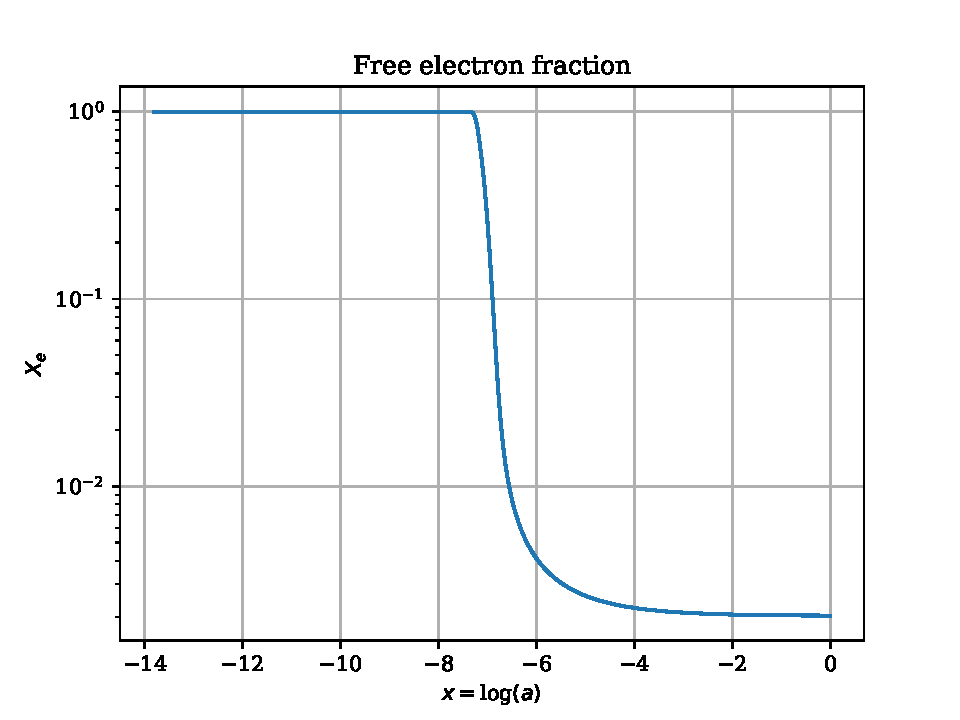
\includegraphics[scale=0.8]{figures/xe.pdf}
    \caption{Figure showing the free electron fraction $X_e$ as a function of $x=log(a)$. The figure shows the solution using both the Saha and the Peebles equation as described in section \ref{sec:method}. Plott as two dots it also illustrated the point of recombination where $X_e=0.5$ for both solutions.}
    \label{fig:xe}
\end{figure}

\begin{figure}
    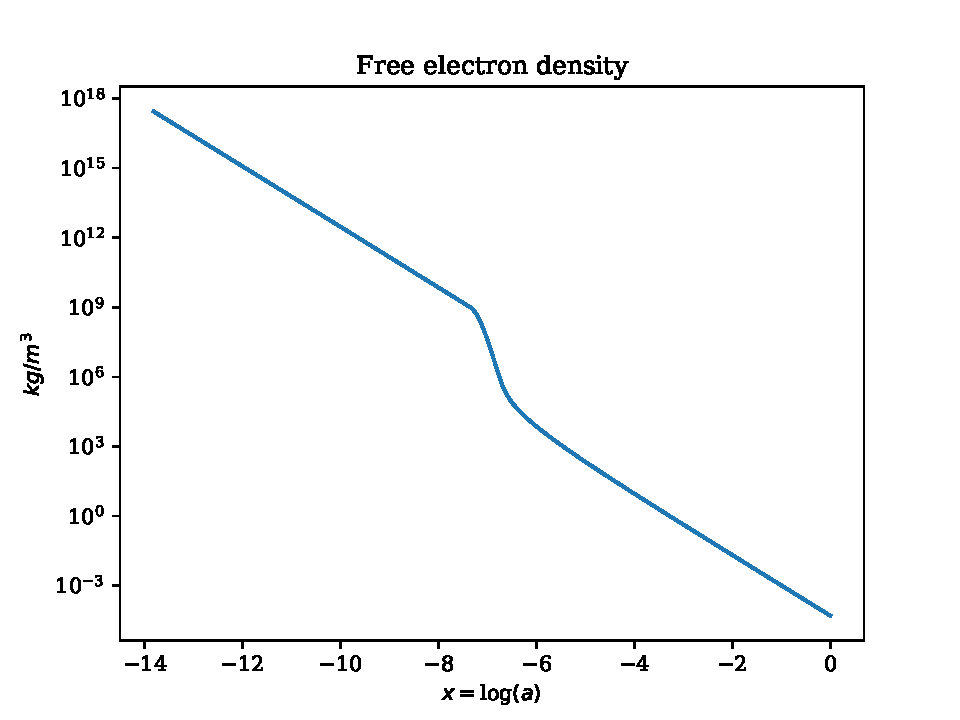
\includegraphics[scale=0.8]{figures/ne.pdf}
    \caption{Figure showing the free electron density $n_e$ as a function of $x=log(a)$.}
    \label{fig:ne}
\end{figure}
The solution for the optical depth $\tau$, calculated by using the expression given by equation \ref{eq:optical_depth_of_x} is shown in figure \ref{fig:tau}.
The visibility function calculated by equation \ref{eq:visibility} is illustraded figure \ref{fig:g}. Furthermore its derivatives are shown in figures \ref{fig:dgdx} and \ref{fig:ddgdxx}.
By the defining the last scattering surface to be the peak of the visibility function, we find the time of the last scattering surface to correspond to $x=-6.98$ which corresponds to an approximate redshift of $z=1077$.
\begin{figure}
    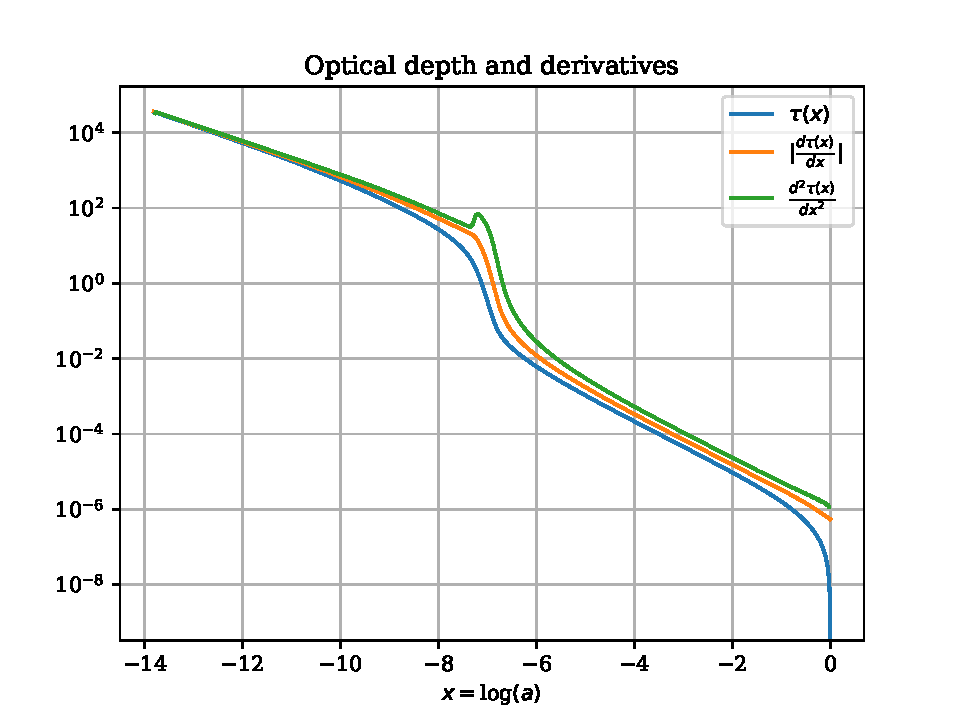
\includegraphics[scale=0.8]{figures/tau.pdf}
    \caption{Figure showing the optical depth of the universe $\tau$ and its derivatives as a function of $x=log(a)$.}S
    \label{fig:tau}
\end{figure}

\begin{figure}
    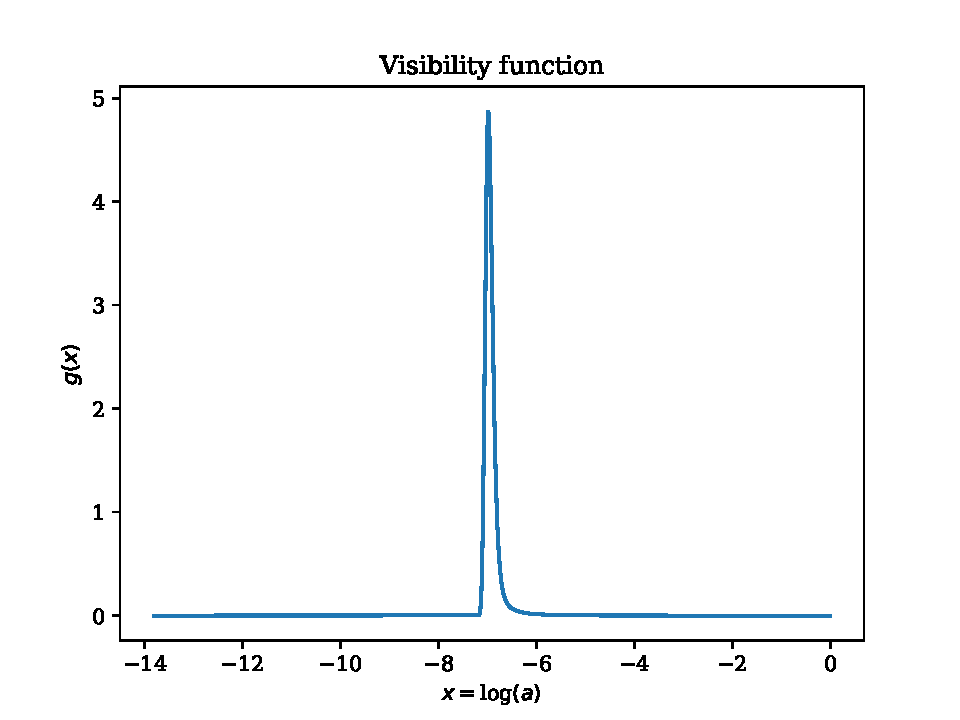
\includegraphics[scale=0.8]{figures/g.pdf}
    \caption{Figure showing the visibility function $\widetilde{g}(x)$ as a function of $x=log(a)$.}
    \label{fig:g}
\end{figure}

\begin{figure}
    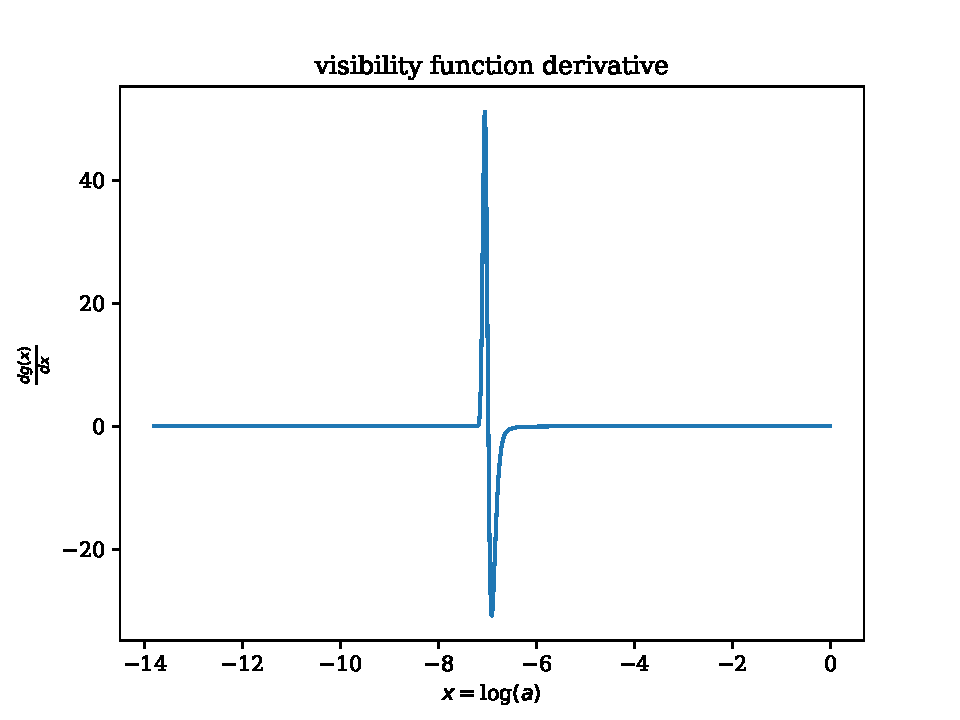
\includegraphics[scale=0.8]{figures/dgdx.pdf}
    \caption{Figure showing the derivative of the visibility function $\frac{d\widetilde{g}(x)}{dx}$ as a function of $x=log(a)$.}
    \label{fig:dgdx}
\end{figure}

\begin{figure}
    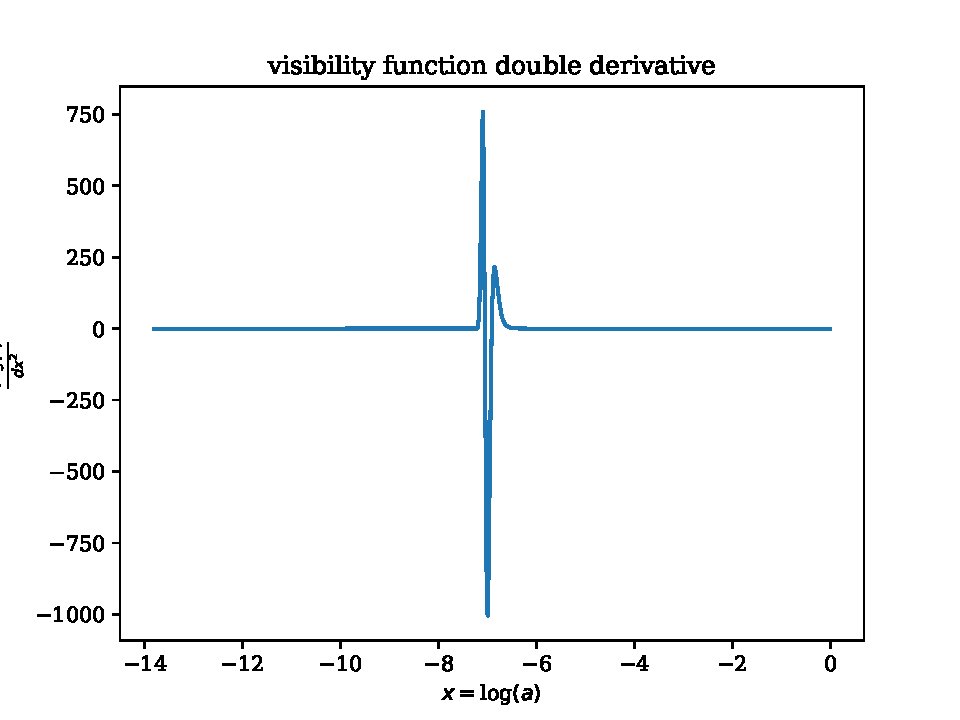
\includegraphics[scale=0.8]{figures/ddgdxx.pdf}
    \caption{Figure showing the double derivative of the visibility function $\frac{d^2\widetilde{g}(x)}{dx^2}$ as a function of $x=log(a)$.}
    \label{fig:ddgdxx}
\end{figure}
As a short benchmark the elapsed time for one random calculation of $X_e$ turned out be $0.00549402$ sec and for $\tau$ the elapsed time was $0.000820157$ sec. All timed with the C++ Chrono library.
\section{Discussion}\label{sec:discussion}
When studying the solution for the free electron fraction, as shown in figure \ref{fig:xe}, one can clearly see that in the early universe all electrons are free. The equilibrium solution from the Saha equation is valid until approximately $x=7.5$. At this time the Saha equation is no longer valid as we no longer have thermal equilibrium due to the expansion of the universe. This allows protons and electron to combine and form neutral hydrogen. The results of our simulations also point to recombination and the last scattering happening shortly after this. We can also see that the solution using only the Saha equation predicts the time of recombination to be close to the combined solution. Allthough it predicts it to happen a bit early. It is also clear from figure \ref{fig:Xe} that the Saha equation is not sufficient to describe the physical conditions after recombination. Shortly after recombination, as seen from the combined solution, electrons freeze out and stabilize at a constant fraction of around $X_e\approx10^{-4}$ making almost all baryonic matter in the universe neutral. By studying the number density of free electrons, as shown in figure \ref{fig:ne}, one can see that the number density experiences a sudden drop around the same time as recombination. Before this the number density falls of exponentially proportional to $a^{-3}$ After recombination, when the free electron fraction has stabilized at a constant value again, the number density of electrons falls off proportional to $a^{-3}$ again.\\\\\indent
When studying the solution for the optical depth, as shown in figure \ref{fig:tau}, one can see that the optical depth increases as we look further back through the universe. After recombination, when the free electon fraction has stabilized, the optical depth increases exponentially. As we look further back in time the universe becomes denser, as shown in the solution for $n_e$, making the scattering on free electrons occur more frequently. During recombination the free electron fraction and the free electron density experiences a dramatic change. This is also reflected on the optical depth. The universe doesn't become optically thick meaning $\tau>1$ untill before recombination has occured. After this The universe is a lot denser and the free electron fraction shows that the universe is almost fully ionized making scattering of free electrons inevitable. One can clearly see that before recombination we have $\tau\gg 1$ making the universe completely opaque. The visibility function $\widetilde{g}(x)$, as shown in figure \ref{fig:g}, peaks at $x=-6.98$ in our simulation. This gives a good estimate to when the last scattering surface occured. This is consistent with the other plots for $X_e$, $n_e$ and $\tau$. It also shows that the last scattering surface occured a small bit after recombination in which we have defined as $X_e=0.5$. This is reasonable as recombination has to occure before thomson scattering due to free electrons becomes negligible. \\\\\indent
We have simulated the process of recombination using a simplified model. Allthough excluding helium, we have a model that produces results consistent with observations and theory. Our model seem to capture the process of last scattering and recombination, allthough excluding reionization our model will propbably not reproduce observed behavior at later times. A further improvement on our model would be to include this in our simulation.




\bibliography{ref.bib}
\bibliographystyle{aasjournal}
%\begin{thebibliography}{}
%\end{thebibliography}
\end{document}

% End of file `sample62.tex'.
